\subsection{Laufzeit \dcsecondauthorshort}
\label{ssec:evaluation:messungen:laufzeit}
Dieser Paragraph beschäftigt sich mit der Ermittlung der maximal verarbeitbaren Bildfrequenz. Durch die Auswertung der Laufzeit der Bildverarbeitungs- und  Regelungskomponente soll die Aufrufhäufigkeit dieser Funktionen so eingestellt werden, dass durch volle Ausnutzung der zur Verfügung stehenden Rechenzeit die schnellstmögliche sichere Fahrt im Testszenario möglich wird.
Außerdem soll der Bestandteil der Bildverarbeitungsfunktion mit dem größten Zeitbedarf identifiziert und, wenn möglich, durch Parameteranpassung oder minimale Quellcodeeingriffe optimiert werden.

%Wichtige, noch anzupassende Parameter stellen dar:
%\begin{itemize}
%\item Die Frequenz, in der Bilder verarbeitet werden
%\item Die Frequenz, mit der die Regelung stattfindet
%\item Die Entfernung des Zielpunktes der Regelung vom Fahrzeug
%\end{itemize}

Den Ausganspunkt für die folgenden Optimierungen bildet eine Geschwindigkeit von
\SI{0.1}{\metre\per\second}. Die Frequenz \scl{f_{img}}, mit welcher die Bilder verarbeitet werden, wurde auf \SI{1}{\hertz} festgelegt, da die Extraktion der Linienpunkte eines Testbildes ca. \SI{0.5}{\second} benötigt. Die Frequenz der Regelung \scl{f_{odom}} wurde initial auf \SI{20}{\hertz} festgelegt, da der Rechenaufwand für einen Regelungszyklus sehr gering ist. Eine noch höhere Regelfrequenz verspricht keinen Performancegewinn und läge schon nahe der maximalen Ansteuerfrequenz des Lenkservos sowie der Abtastrate der \gls{acr:imu} (jeweils \SI{50}{\hertz}).

Mithilfe dieser Einstellung absolvierte das Fahrzeug erfolgreich eine Runde im Testparcours. Wie in Abb.~\ref{fig:evaluation:riverflow:times_combined_1Hz_0_1m_s_over_piciter} zu sehen, benötigt ein Bild-Callback im Echtzeitbetrieb, d.h. bei mehrmaliger Ausführung erheblich weniger Zeit als bei einmaliger Messung anhand eines Testbildes. Die Verringerung der Bearbeitungsdauer \scl{t_{img}} von ca. \SI{500}{\milli\second} auf \SI{128}{\milli\second} (Median der in Abb.~\ref{fig:evaluation:riverflow:times_combined_1Hz_0_1m_s_over_piciter} dargestellten Daten) lässt sich unter anderem durch die Fahigkeit MATLABs, Funktionen bei wiederholter Ausführung im Hauptspeicher zu halten und somit schneller ausführen zu können, erklären. Eine signifikante Erhöhung der Bildfrequenz \scl{f_{img}} ist also möglich. Nimmt man die von der Regelung und Posenaktualisierung, d.h. dem Odometrie-Callback benötigte Zeit als konstant an, lässt sich die theoretisch mögliche Bildfrequenz wie folgt berechnen:
\begin{subequations}
\begin{equation}
	T_{img} = t_{img}+t_{odom-per-sec}\cdot T_{img}
\end{equation}
%\begin{equation}
%	T_{img}\cdot(1-t_{odom-per-sec}) = t_{img}
%\end{equation}
\begin{equation}
	T_{img} = \frac{t_{img}}{1-t_{odom-per-sec}}
\end{equation}
\begin{equation}	
	f_{img} = \frac{1}{T_{img}}
\end{equation}
\end{subequations} 
Die vom Odometrie-Callback pro Sekunde in Anspruch genommene Zeit \scl{t_{odom-per-sec}} wurde direkt als Median der in Abb.~\ref{fig:evaluation:riverflow:times_combined_1Hz_0_1m_s_over_piciter} dargestellten Messwerte errechnet, könnte aber bei einer von \SI{1}{\hertz} abweichenden initialen Bildfrequenz auch auf Basis der Dauer eines Odometrie-Callbacks \(t_{odom}\) bestimmt werden: 
\begin{equation}
t_{odom-per-sec} = t_{odom} \cdot f_{odom}
\end{equation}
Mit einer Bildbearbeitungszeit von \(t_{img}=\SI{128}{\milli\second}\) sowie dem Zeitbedarf des Odometrie-Callbacks von \(t_{odom-per-sec}=\SI{262}{\milli\second\per\second}\), ergibt sich eine in der Theorie nutzbare Framerate von über \SI{5}{\hertz}. Mit dieser Bildfrequenz wurde eine weitere Testfahrt absolviert, in Abb. \ref{fig:evaluation:riverflow:times_pic_5Hz_0_2m_s_over_piciter} wird die bessere Nutzung der zur Verfügung stehenden Rechenzeit deutlich. Abbildung \ref{fig:evaluation:riverflow:times_pic_5Hz_0_2m_s_over_piciter} zeigt jedoch auch, dass die Periodendauer der Bildverarbeitung zwischen 2 Punkten oszilliert. Der erwartete zeitliche Abstand zweier konsekutiver Aufnahmen von \SI{200}{ms} wird häufig nicht erreicht, stattdessen befindet sich ein Abstand von \(2 \cdot \SI{200}{ms} = \SI{400}{ms}\) zwischen aufeinander folgenden Bildern. Dies führt zu dem Schluss, dass durch nicht vorhandene, da kontraproduktive Pufferung Aufnahmen ausgelassen wurden.

\begin{figure}[htbp] % [htb]
\centering
\subfloat[\SI{5}{\hertz}\label{fig:evaluation:riverflow:times_pic_5Hz_0_2m_s_over_piciter}]{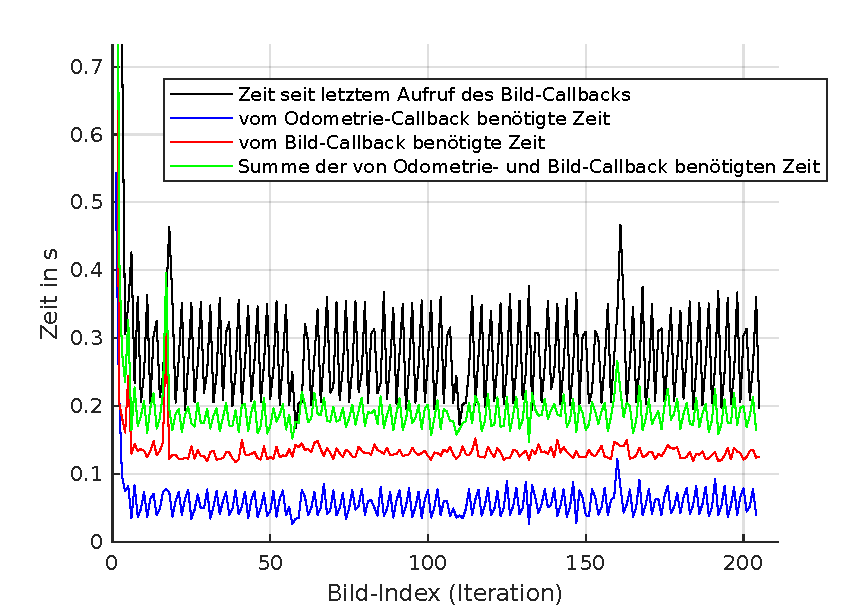
\includegraphics[scale=\mtlstscale]{evaluation_riverflow_times_combined_5Hz_0_2m_s_over_piciter}}
\hfill
\subfloat[\SI{4}{\hertz}\label{fig:evaluation:riverflow:times_pic_4Hz_0_2m_s_over_piciter}]{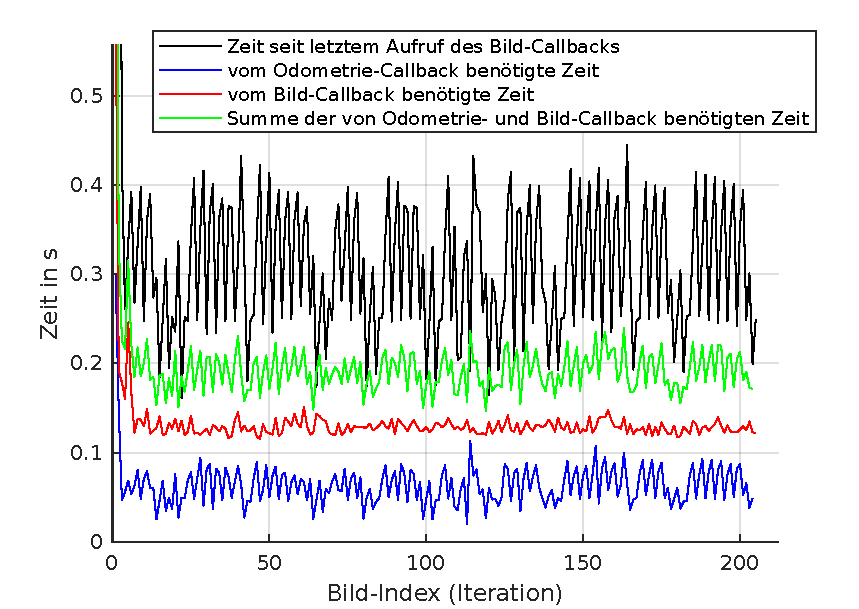
\includegraphics[scale=\mtlstscale]{evaluation_riverflow_times_combined_4Hz_0_2m_s_over_piciter}}
\hfill
\subfloat[\SI{3}{\hertz}\label{fig:evaluation:riverflow:times_pic_3Hz_0_2m_s_over_piciter}]{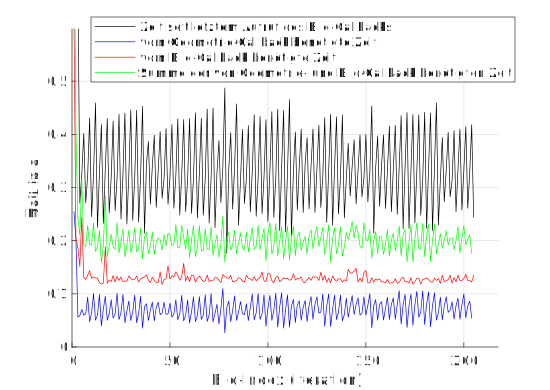
\includegraphics[scale=\mtlstscale]{evaluation_riverflow_times_combined_3Hz_0_2m_s_over_piciter}}
\hfill
\subfloat[\SI{1}{\hertz}\label{fig:evaluation:riverflow:times_combined_1Hz_0_1m_s_over_piciter}]{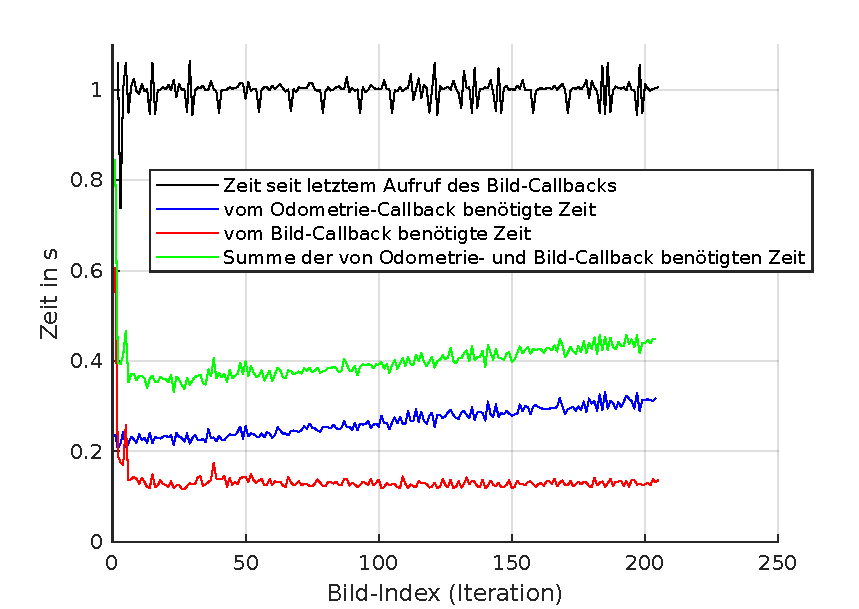
\includegraphics[scale=\mtlstscale]{evaluation_riverflow_times_combined_1Hz_0_1m_s_over_piciter}}
\caption{Zeitbedarf aller Fahrspurverfolgungskomponenten bei \SIlist{5;4;3;1}{\hertz} Bildfrequenz}
\end{figure}

Im Folgenden wurde die Bildfrequenz zuerst auf 4 (s.~Abb.~\ref{fig:evaluation:riverflow:times_pic_4Hz_0_2m_s_over_piciter}), später auf \SI{3}{\hertz} verringert (s.~Abb.~\ref{fig:evaluation:riverflow:times_pic_3Hz_0_2m_s_over_piciter}). Erst jetzt konnte kein Springen der Periodendauer des Bild-Callbacks auf ein Vielfaches seines Erwartungswertes mehr festgestellt werden. Eine leichte Oszillation des zeitlichen Abstands zweier Aufnahmen ist auch in Abb.~\ref{fig:evaluation:riverflow:times_pic_3Hz_0_2m_s_over_piciter} zu erkennen, jedoch beträgt der Mittelwert fast exakt die erwarteten \SI{333}{ms}. Die verbleibenden Unregelmäßigkeiten sind auf den Kamera-Node, welcher die Bilder aufnimmt und im entsprechenden Topic veröffentlicht, zurückzuführen (s. Abb.~\ref{fig:evaluation:riverflow:times_pic_3Hz_0_2m_s_since_matlab_ros} und Abschnitt \ref{ssec:software_struktur:ros:nodes}). Abbildung \ref{fig:evaluation:riverflow:times_combined_3Hz_0_2m_s_pie_median} 
% bzw. \ref{fig:evaluation:riverflow:times_combined_3Hz_0_2m_s_pie_mean} 
stellt zusammenfassend die pro Bild mit Regelung, Bildverarbeitung, sonstigem Overhead \&\ im Leerlauf verbrachte Zeit einer gefahrenen Runde dar.

\begin{figure}[htbp]
\centering
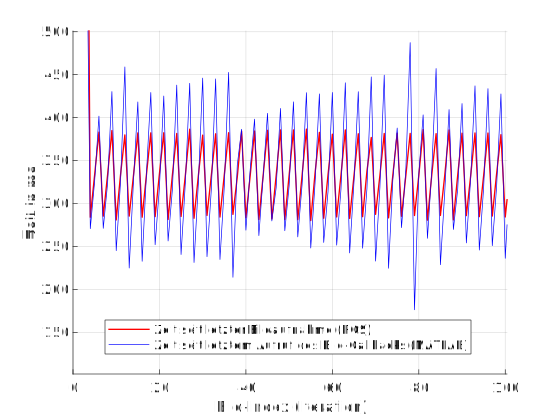
\includegraphics[scale=\mtlstscale]{evaluation_riverflow_times_pic_3Hz_0_2m_s_since_matlab_ros}
\caption{Schwankungen Periodendauer Bildaufnahme/Bild-Callback bei \SI{3}{\hertz} Bildfrequenz}
\label{fig:evaluation:riverflow:times_pic_3Hz_0_2m_s_since_matlab_ros}
\end{figure}

\begin{figure}[htbp] % [htb]
	\centering
	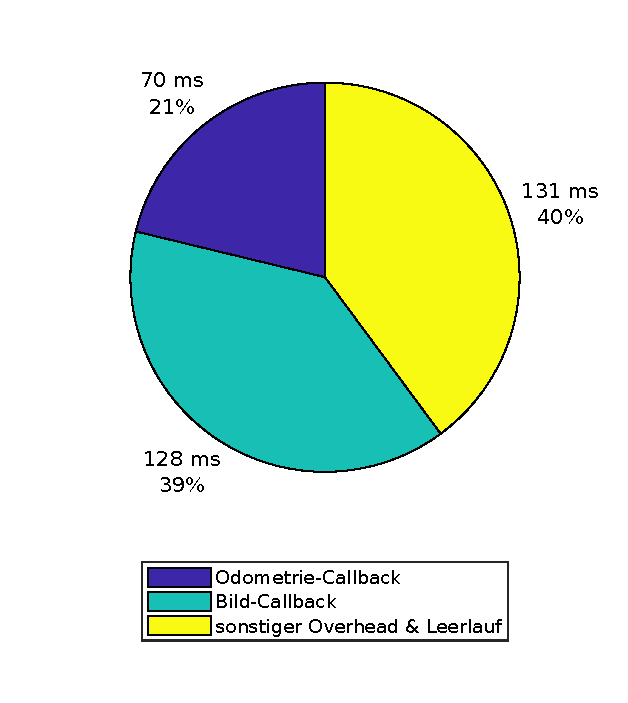
\includegraphics[scale=\mtlstscale]{evaluation_riverflow_times_combined_3Hz_0_2m_s_pie_median}
	\caption{Zeitbedarf aller Fahrspurverfolgungskomponenten pro Aufnahme bei \SI{3}{\hertz} Bildfrequenz; Median aller Messwerte einer Runde der Teststrecke}
	\label{fig:evaluation:riverflow:times_combined_3Hz_0_2m_s_pie_median}
\end{figure}

%\begin{figure}[htbp] % [htb]
%	\centering
%	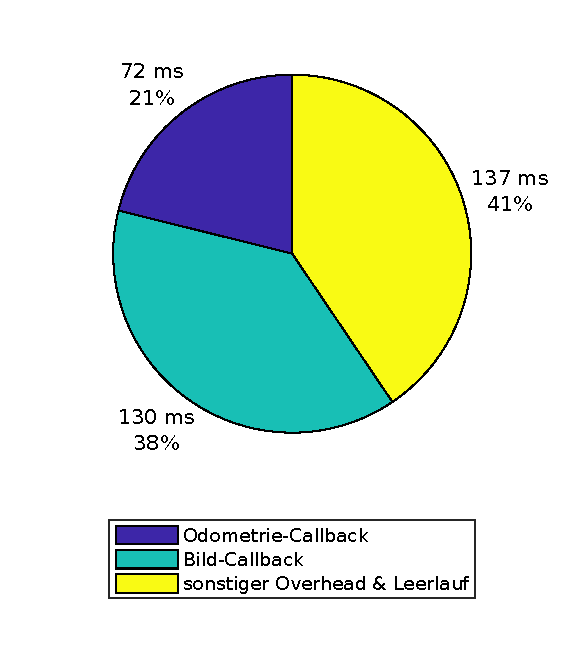
\includegraphics[scale=\mtlstscale]{evaluation_riverflow_times_combined_3Hz_0_2m_s_pie_mean}
%	\label{fig:evaluation:riverflow:times_combined_3Hz_0_2m_s_pie_mean}
%	\caption{Zeitbedarf aller Fahrspurverfolgungskomponenten bei \SI{3}{\hertz} Bildfrequenz; Mittelwert aller Messwerte einer Runde der Teststrecke}
%\end{figure}

\paragraph{Dauer einzelner Komponenten der Fahrspurerkennung}
Um in Zukunft Optimierungen an den implementierten Bildverarbeitungsalgorithmen durchführen zu können, ist es unumgänglich, nicht nur die gesamt benötigte Zeit, sondern auch die Dauer der einzelnen Module zu messen.

\begin{figure}[htbp] % [htb]
\centering
\subfloat[Boxplot\label{fig:evaluation:riverflow:times_pic_3Hz_0_2m_s_boxplot}]{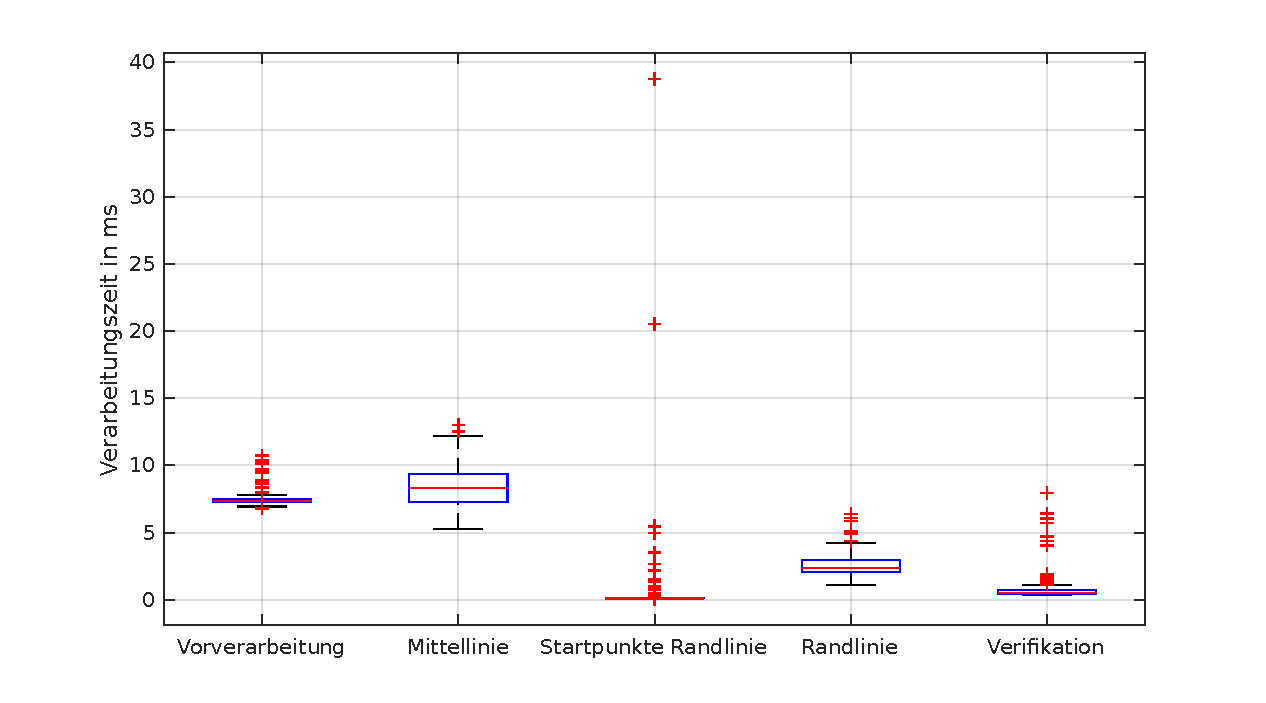
\includegraphics[scale=\mtlstscale]{evaluation_riverflow_times_pic_3Hz_0_2m_s_boxplot}}
% ohne Startphase
\hfill	
%\subfloat[Boxplot ohne Startphase\label{fig:evaluation:riverflow:times_pic_3Hz_0_2m_s_boxplot_ros}]{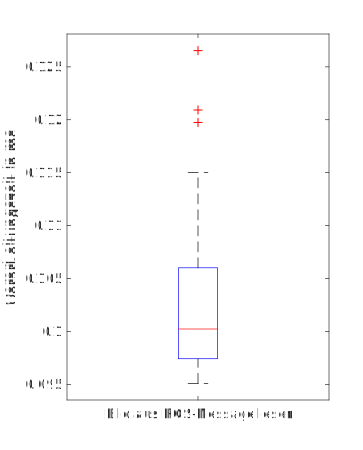
\includegraphics[scale=\mtlstscale]{evaluation_riverflow_times_pic_3Hz_0_2m_s_boxplot_ros}}
%\hfill
\subfloat[Tortendiagramm; Median aller Messwerte einer Runde\label{fig:evaluation:riverflow:times_pic_3Hz_0_2m_s_pie_no_ros}]{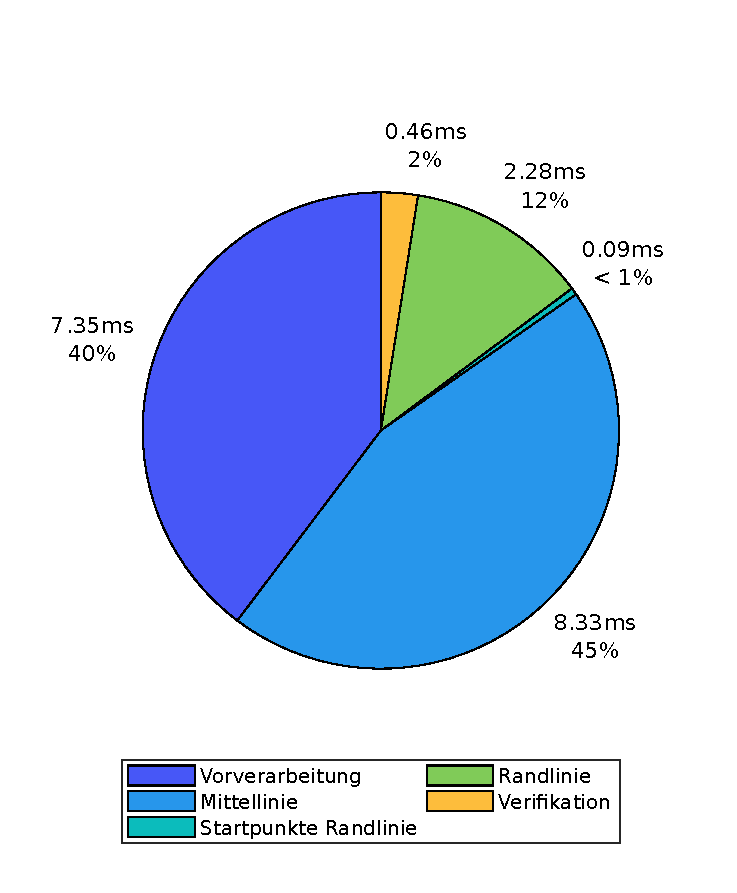
\includegraphics[scale=\mtlstscale]{evaluation_riverflow_times_pic_3Hz_0_2m_s_pie_no_ros}}
\hfill
%Summe:18.5185ms	
\subfloat[Tortendiagramm; Median aller Messwerte einer Runde; mit Dekompression des Bildes\label{fig:evaluation:riverflow:times_pic_3Hz_0_2m_s_pie_with_ros}]{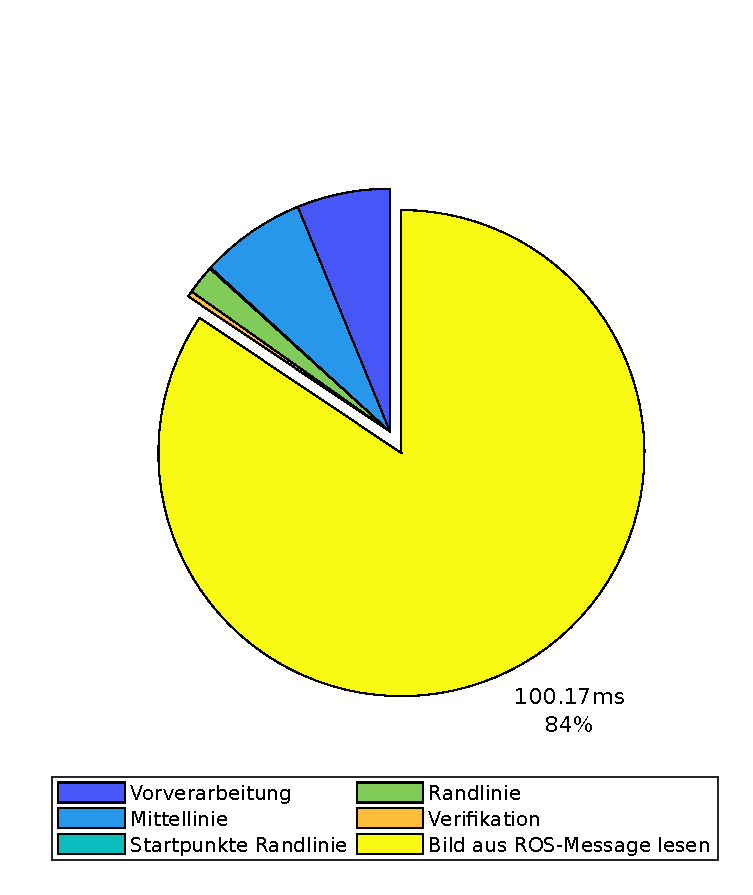
\includegraphics[scale=\mtlstscale]{evaluation_riverflow_times_pic_3Hz_0_2m_s_pie_with_ros}}
\caption{Zeitbedarf aller Fahrspurerkennungskomponenten bei \SI{3}{\hertz} Bildfrequenz}
\end{figure}

Diese Untersuchungen führten zu interessanten Ergebnissen, welche die Echtzeitfähigkeit der MATLAB-\gls{acr:ros}-Schnittstelle in Frage stellen. Wie in Abbildung \ref{fig:evaluation:riverflow:times_pic_3Hz_0_2m_s_pie_with_ros} zu sehen, wird ein Großteil der Dauer eines Bild-Callbacks zum Umwandeln der \gls{acr:ros}-Message in eine von MATLAB prozessierbare Matrix benötigt. Eine genauere Untersuchung mit dem MATLAB-Profiler zeigte, dass in diesem Schritt eine Dekompression des im JPEG-Format übertragenen Bildes den wesentlichen Anteil dieses Zeitbedarfs verursacht. Eine unkomprimierte Übertragung würde jedoch ein vielfaches dieser Dauer in Anspruch nehmen.

Der eigens entwickelte Anteil der Fahrspurerkennung benötigt im Median einer Runde lediglich \SI{18,5}{ms}, die genaue Aufteilung kann in Abb. \ref{fig:evaluation:riverflow:times_pic_3Hz_0_2m_s_pie_no_ros} sowie \ref{fig:evaluation:riverflow:times_pic_3Hz_0_2m_s_boxplot} nachvollzogen werden. Die meiste Zeit wird für Bildvorverarbeitung und Mittellinienerkennung benötigt. Da diese Funktionen zum Großteil auf vorgegebenen, komplexen und bereits maschinennah implementierten MATLAB-Funktionen basieren, kann hier nur unter Nutzung anderer Software eine Optimierung stattfinden. Die zum Großteil aus elementaren Funktionen aufgebaute Erkennung \&\ Verifikation der Randlinie läuft schon hinreichend schnell ab, sodass hier trotz der vielen verwendeten, in MATLAB rechenzeitintensiven Schleifen keine effizientere Alternative gesucht werden muss.

\subparagraph{Startpunktfindung}
Wie in Abb.~\ref{fig:evaluation:riverflow:times_pic_3Hz_0_2m_s_pie_no_ros} zu sehen, verstreicht im Normalfall bei der Feststellung der Startpunkte zur Erkennung der seitlichen Fahrbahnmarkierungen kaum Zeit. Wird jedoch kein Mittellinienelement nahe genug vor dem Fahrzeug gefunden, so gestaltet sich dieser Prozess aufwendiger (siehe Abschnitt~\ref{sssec:fahrspurerkennung:riverflow:randlinie:startpunktgewinnung}). Abbildung~\ref{fig:evaluation:riverflow:times_startpoints_3Hz_0_2m_s_boxplot} gibt ein besseres Bild der Messwerte wieder als Diagramm \ref{fig:evaluation:riverflow:times_pic_3Hz_0_2m_s_pie_no_ros} bzw. \ref{fig:evaluation:riverflow:times_pic_3Hz_0_2m_s_boxplot}, da hier nicht nur der Median aller Messwerte gebildet, sondern vor der Erstellung des Boxplots die Daten nach der Methode zur Startpunktbestimmung sortiert wurden. 
\begin{figure}[htbp] % [htb]
\centering
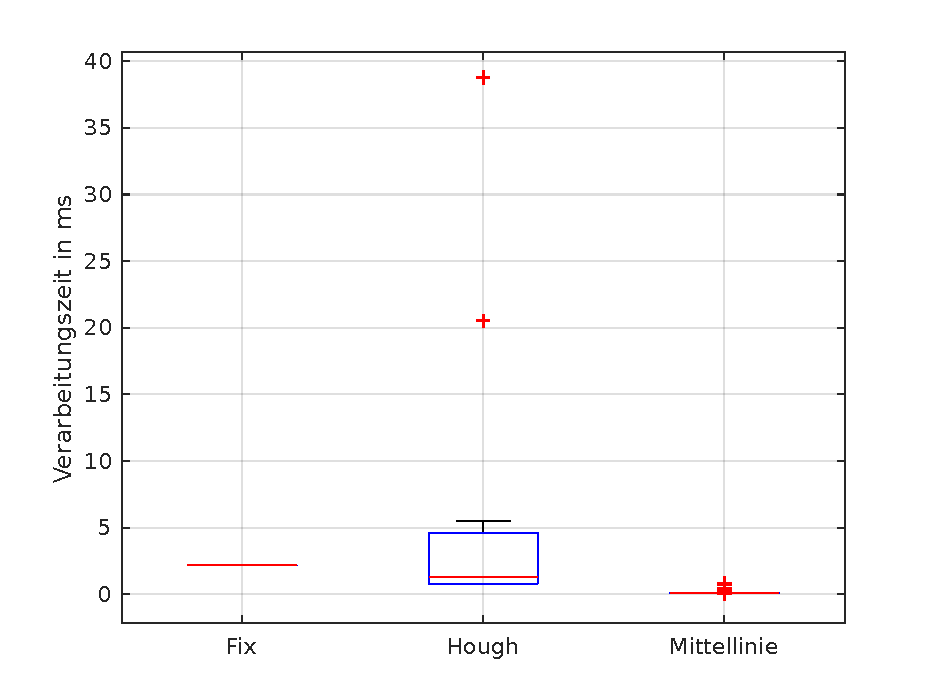
\includegraphics[scale=\mtlstscale]{evaluation_riverflow_times_startpoints_3Hz_0_2m_s_boxplot}
\caption{Zeitbedarf der Startpunktfindungsalgorithmen für die Erkennung der seitlichen Fahrbahnmarkierungen bei \SI{3}{\hertz} Bildfrequenz}
\label{fig:evaluation:riverflow:times_startpoints_3Hz_0_2m_s_boxplot}
\end{figure}
Die Erwartung, dass bei Nutzung der mittigen Fahrbahnmarkierung zur Startpunktgenerierung kaum Zeit vergeht, wurde durch den über diese Kategorie gebildeten Median von \SI{0,09}{ms} bestätigt. Jedoch ist auch die von der eindimensionalen Hough-Transformation im Median benötigte Laufzeit von \SI{1,32}{ms} vertretbar. Die in Abbildung \ref{fig:evaluation:riverflow:times_startpoints_3Hz_0_2m_s_boxplot} sichtbaren Ausreißer entstehen durch das erstmalige Ausführen der Funktion, welche nicht während der im Boxplot unberücksichtigten \glqq Warmlaufphase\grqq\ geschieht. Da nur einmal fix im Bildkoordinatensystem liegende Punkte genutzt werden mussten und dieser Fall nur nach Fehlschlag der eindimensionalen Hough-Transformation auftritt, wird dieser Messwert nur als Median ohne Box etc. in Abb. \ref{fig:evaluation:riverflow:times_startpoints_3Hz_0_2m_s_boxplot} dargestellt und bewegt sich mit \SI{2,17}{ms} im Bereich dieser Methode.

\paragraph{Übertragungszeit}
Durch JPEG-Kompression mit einer Qualitätseinstellung von 20\% wurde der Bildtransfer ohne großen Informationsverlust auf \SI{77,2}{ms} im Median beschleunigt (s. Abb. \ref{fig:evaluation:riverflow:times_pictransfer_3Hz_0_2m_s_boxplot}). Diese Übertragungszeit stellt immer noch eine erhebliche Totzeit dar, lässt sich aufgrund der hohen benötigten Rohdatenauflösung von 1080x1080 Pixeln ohne grundsätzliche Änderung des verwendeten Hardwareaufbaus und der Softwarestruktur jedoch nicht weiter verringern. Die Streuung der Messwerte bis hin zu \SI{183}{ms} spiegelt die Probleme der Nutzung einer WLAN-Verbindung, welche zu unvorhersehbaren Latenzen neigt, wieder.
Die angesprochene Totzeit schlägt sich jedoch nicht direkt auf das Fahrverhalten des Modellautos nieder, da die Bildverarbeitung wie in Passage \ref{ssec:software_struktur:matlab:callbacks} beschrieben getrennt von der Regelung des Roboters abläuft.

\begin{figure}[htbp] % [htb]
\centering
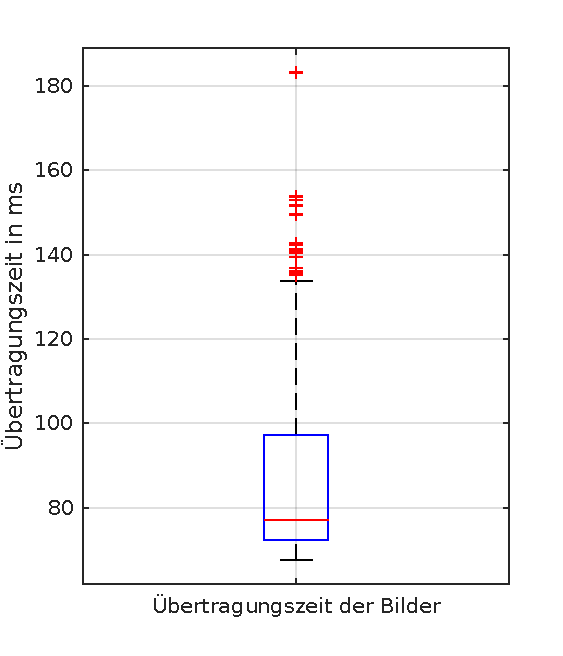
\includegraphics[scale=\mtlstscale]{evaluation_riverflow_times_pictransfer_3Hz_0_2m_s_boxplot}
\caption{Übertragungszeit der Aufnahmen bei \SI{3}{\hertz} Bildfrequenz}
\label{fig:evaluation:riverflow:times_pictransfer_3Hz_0_2m_s_boxplot}
\end{figure}
